\documentclass{article}
\usepackage[utf8]{inputenc}

\title{Assignment 1}
\author{Siddharth Nayak EE16B073}
\date{10th September 2018}
%\note{Please do not share:The project work will be submitted as a research paper }

\usepackage{natbib}
\usepackage{graphicx}
\usepackage{geometry}
\geometry{legalpaper, portrait, margin=1.5in}
\usepackage{sidecap}
\usepackage{graphicx}
\usepackage{subcaption}
\usepackage[section]{placeins}

\begin{document}

\maketitle

\section{Introduction}
The Hodgkin-Huxley model explains how the dynamics of ion channels (Na+, K+ etc) contribute to the generation of an Action Potential in a neuron.\\
An Action Potential is a sharp voltage spike elicited by stimulating a neuron with a current that exceeds a certain threshold value. The current amplitude is increased gradually, at a threshold amplitude, the voltage response does not increase proportionally. \\
It shows a sharp, disproportionate increase.\\ Once the membrane voltage reaches a threshold value, it increase further rapidly to maximum value and drops again rapidly to a value that is less than resting value, before returning to the baseline value after a delay.

 
 \begin{figure}[h]
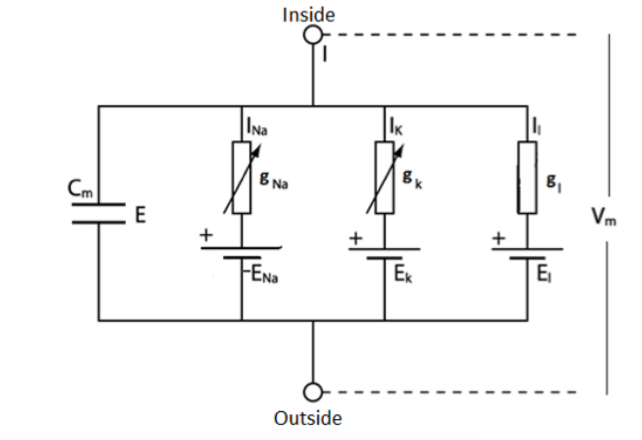
\includegraphics[width=8cm]{circuit.png}
\caption{Hodgkin-Huxley model circuit}

\end{figure}

\section{Results}
The plot of voltage vs time behaves differently for different applied external current. At some particular values of input current even a small change causes the system dynamics to change a lot.\\
For input current ranging from 0$\mu$A to 0.02235$\mu$A we do not get any action potentials.
For a change in input current from 0.02235$\mu$A to 0.02236$\mu$A we suddenly start getting action potentials but they are not periodic.\\
For a change in input current from 0.0622$\mu$A to 0.06223$\mu$A we suddenly start getting periodic action potentials.\\
For a change in input current from 0.450$\mu$A to 0.451$\mu$A we stop getting action potentials(i.e. assuming if peak voltage is below 10mV then we do not consider it as an action potential).

\section{Frequency vs Input current}
As we can see in the obtained plots, we start getting periodic action potentials from 0.06223$\mu$A to 0.450$\mu$A.\\
Thus we can obtain a frequency vs input current plot for the same. The frequency will be zero initially till 0.0622$\mu$A.\\
After that we get a frequency value at 0.06223$\mu$A and it increases till the input current in increased till 0.450$\mu$A.\\
After 0.450$\mu$A again we get zero frequency as we do not have action potentials.
\newpage
\section{Region 1}
\begin{figure}[h]
    \centering
    \begin{subfigure}[b]{0.5\textwidth}
        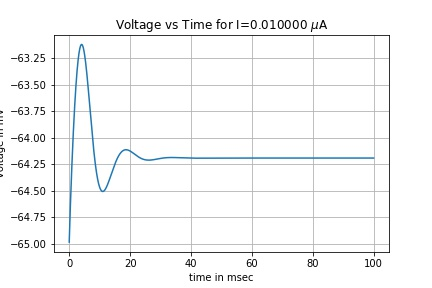
\includegraphics[width=\textwidth]{1.jpg}}
        \caption{Plot of Voltage vs Time for I=0.01$\mu$A}
        \label{fig:IOU1}
    \end{subfigure}
    
     %add desired spacing between images, e. g. ~, \quad, \qquad, \hfill etc. 
      %(or a blank line to force the subfigure onto a new line)
    \begin{subfigure}[b]{0.5\textwidth}
        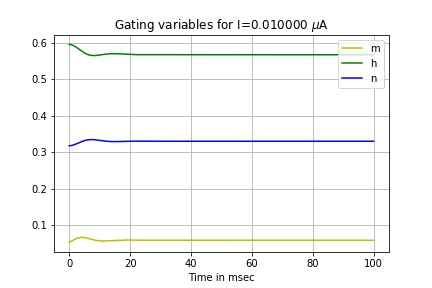
\includegraphics[width=\textwidth]{2.jpg}}
        \caption{Plot of gating variables for I=0.01$\mu$A}
        \label{fig:IO2}
    \end{subfigure}
    %add desired spacing between images, e. g. ~, \quad, \qquad, \hfill etc. 
    %(or a blank line to force the subfigure onto a new line)
    \begin{subfigure}[b]{0.5\textwidth}
        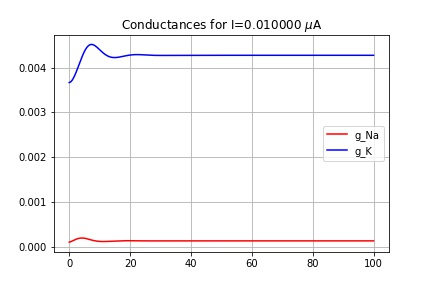
\includegraphics[width=\textwidth]{3.jpg}}
        \caption{Plot of conductances for I=0.01$\mu$A}
        \label{fig:IO2}
    \end{subfigure}
\end{figure}
\newpage
\section{Region 2}

\begin{figure}[h]
    \centering
    \begin{subfigure}[h]{0.5\textwidth}
        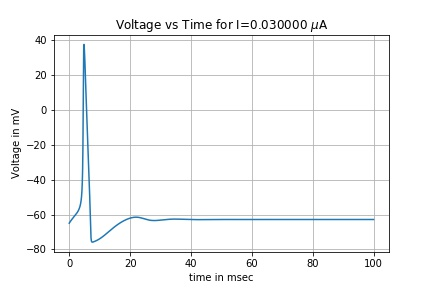
\includegraphics[width=\textwidth]{4.jpg}}
        \caption{Plot of Voltage vs Time for I=0.03$\mu$A}
        \label{fig:IOU1}
    \end{subfigure}
    
     %add desired spacing between images, e. g. ~, \quad, \qquad, \hfill etc. 
      %(or a blank line to force the subfigure onto a new line)
    \begin{subfigure}[b]{0.5\textwidth}
        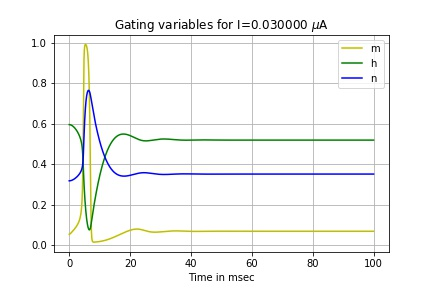
\includegraphics[width=\textwidth]{5.jpg}}
        \caption{Plot of gating variables for I=0.03$\mu$A}
        \label{fig:IO2}
    \end{subfigure}
    %add desired spacing between images, e. g. ~, \quad, \qquad, \hfill etc. 
    %(or a blank line to force the subfigure onto a new line)
    \begin{subfigure}[b]{0.5\textwidth}
        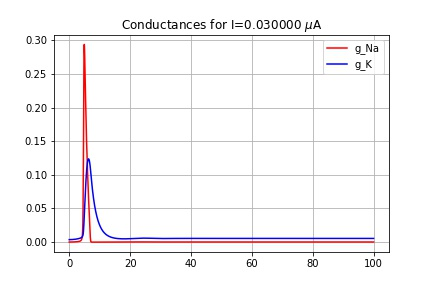
\includegraphics[width=\textwidth]{6.jpg}}
        \caption{Plot of conductances for I=0.03$\mu$A}
        \label{fig:IO2}
    \end{subfigure}
\end{figure}
\newpage
\section{Region 3}

\begin{figure}[h]
    \centering
    \begin{subfigure}[b]{0.5\textwidth}
        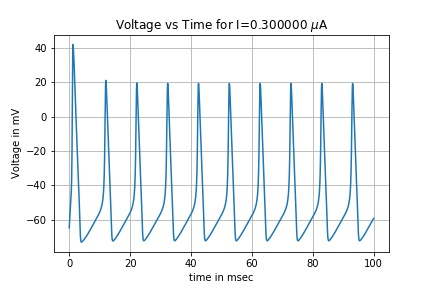
\includegraphics[width=\textwidth]{7.jpg}}
        \caption{Plot of Voltage vs Time for I=0.3$\mu$A}
        \label{fig:IOU1}
    \end{subfigure}
    
     %add desired spacing between images, e. g. ~, \quad, \qquad, \hfill etc. 
      %(or a blank line to force the subfigure onto a new line)
    \begin{subfigure}[b]{0.5\textwidth}
        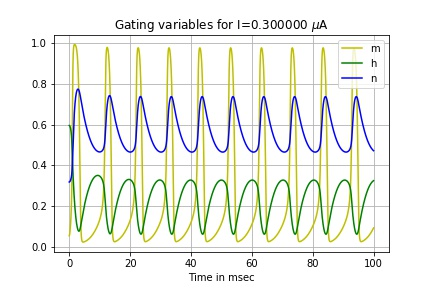
\includegraphics[width=\textwidth]{8.jpg}}
        \caption{Plot of gating variables for I=0.3$\mu$A}
        \label{fig:IO2}
    \end{subfigure}
    %add desired spacing between images, e. g. ~, \quad, \qquad, \hfill etc. 
    %(or a blank line to force the subfigure onto a new line)
    \begin{subfigure}[b]{0.5\textwidth}
        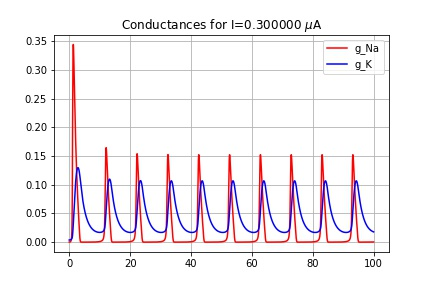
\includegraphics[width=\textwidth]{9.jpg}}
        \caption{Plot of conductances for I=0.3$\mu$A}
        \label{fig:IO2}
    \end{subfigure}
\end{figure}
\newpage
\section{Region 4}

\begin{figure}[h]
    \centering
    \begin{subfigure}[b]{0.5\textwidth}
        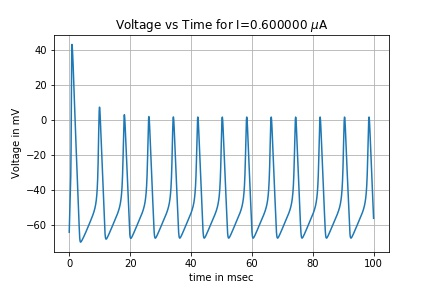
\includegraphics[width=\textwidth]{10.jpg}}
        \caption{Plot of Voltage vs Time for I=0.6$\mu$A}
        \label{fig:IOU1}
    \end{subfigure}
    
     %add desired spacing between images, e. g. ~, \quad, \qquad, \hfill etc. 
      %(or a blank line to force the subfigure onto a new line)
    \begin{subfigure}[b]{0.5\textwidth}
        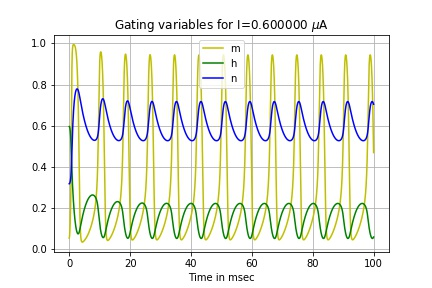
\includegraphics[width=\textwidth]{11.jpg}}
        \caption{Plot of gating variables for I=0.6$\mu$A}
        \label{fig:IO2}
    \end{subfigure}
    %add desired spacing between images, e. g. ~, \quad, \qquad, \hfill etc. 
    %(or a blank line to force the subfigure onto a new line)
    \begin{subfigure}[b]{0.5\textwidth}
        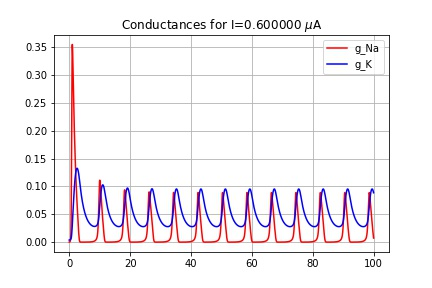
\includegraphics[width=\textwidth]{12.jpg}}
        \caption{Plot of conductances for I=0.6$\mu$A}
        \label{fig:IO2}
    \end{subfigure}
\end{figure}




\newpage
\section{Frequency vs Input current plot}
We have zero frequency before and after Region 3.

 \begin{figure}[h]
 \centering
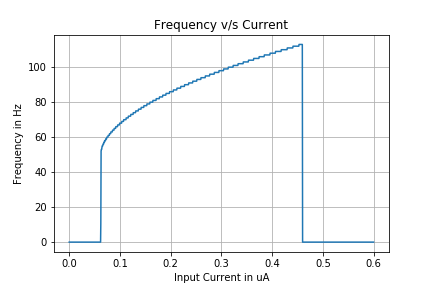
\includegraphics[width=10cm]{freq.png}
\caption{Frequency vs Input current plot}

\end{figure}




%``I always thought something was fundamentally wrong with the universe'' \citep{adams1995hitchhiker}

\bibliographystyle{plain}
\bibliography{references}
\end{document}
